\documentclass[conference]{IEEEtran}
\IEEEoverridecommandlockouts
% The preceding line is only needed to identify funding in the first footnote. If that is unneeded, please comment it out.
\usepackage{cite}
\usepackage{amsmath,amssymb,amsfonts}
\usepackage{algorithmic}
\usepackage{graphicx}
\usepackage{textcomp}
\usepackage{xcolor}
\def\BibTeX{{\rm B\kern-.05em{\sc i\kern-.025em b}\kern-.08em
    T\kern-.1667em\lower.7ex\hbox{E}\kern-.125emX}}
    
% Code formatting
\usepackage{listings}
\usepackage{xcolor}

\definecolor{codegreen}{rgb}{0,0.6,0}
\definecolor{codegray}{rgb}{0.5,0.5,0.5}
\definecolor{codepurple}{rgb}{0.58,0,0.82}
\definecolor{backcolour}{rgb}{0.95,0.95,0.92}

\lstdefinestyle{cpp}{
    backgroundcolor=\color{backcolour},
    commentstyle=\color{codegreen},
    keywordstyle=\color{magenta},
    numberstyle=\tiny\color{codegray},
    stringstyle=\color{codepurple},
    basicstyle=\ttfamily\footnotesize,
    breakatwhitespace=false,
    breaklines=true,
    captionpos=b,
    keepspaces=true,
    numbers=left,
    numbersep=5pt,
    showspaces=false,
    showstringspaces=false,
    showtabs=false,
    tabsize=2
}

\lstset{style=cpp}
    

\begin{document}

\title{Concurrent Graph Algorithms}

\author{\IEEEauthorblockN{Jacob Steinebronn}
\and
\IEEEauthorblockN{Daniel West}
\and
\IEEEauthorblockN{William Quiroga}
\and
\IEEEauthorblockN{Alex Rutledge}}

\maketitle

\begin{abstract}
This document is a model and instructions for \LaTeX.
This and the IEEEtran.cls file define the components of your paper [title, text, heads, etc.]. *CRITICAL: Do Not Use Symbols, Special Characters, Footnotes, 
or Math in Paper Title or Abstract.
\end{abstract}

\begin{IEEEkeywords}
graph, algorithm, dijkstra, floyd-warshall, shortest-path
\end{IEEEkeywords}

\section{Introduction}
In this paper, we will perform a wide analysis on several high-level graph topics: the All-Pairs-Shortest-Path problem, the Minimum Spanning Tree problem, the Shortest-Distance problem with negative edges, and the Disjoint Set Union data structure (which is often used in graph algorithms such as connectivity or Kruskal's MST algorithm). In particular, the implementations of these algorithms in parallel will be analyzed in detail regarding the best practices for different use-cases or input regimes. 
\section{All-Pairs Shortest-Path}

\subsection{Problem Definition}

Given a weighted, undirected graph G, $\forall u, v \in G$, find $DIST_{u,v}$ equal to the shortest path in G from $u$ to $v$. In general, the edge weights can be any real number, but for our purposes it will be convenient to restrict edge weights to non-negative integers which do not exceed $10^9$. This will be done for two main reasons:
\begin{itemize}
    \item To restrict the maximum possible answer into an integer which can be stored conveniently in most modern operating systems (a 64-bit signed integer will suffice)
    \item To restrict the graph such that path lengths are defined. With negative edge weights, a path could simply traverse this negative edge back and forth infinitely many times, so any fully relaxed path in a graph with at least one negative edge weight will have all paths of length $-\infty$
\end{itemize}
These two items let us prove a convenient upper-bound on the length of any one shortest path as follows: Let $w_{max}$ be the largest possible edge weight. Any shortest path from $u$ to $v$, $P = p_0,p_1,...p_{n-1},p_k \,\,|\,\, p_0 = u, p_k = v$ will be simple; that is, there will not exist any node $p_i$ which appears in $P$ twice. We can show this by contradiction: If there were some node that appeared twice in $P$, let the first and last occurrence of this duplicate node be $p_i$ and $p_j$, then $P' = p_0, p_1...p_i,p_{j+1},p_{j+2}...p_k$ would be shorter. That is, we could "cut out" the cycle between $p_i$ and $p_j$. Thus, we know that for any shortest path, every node in G will appear at most once, so the maximum value for any shortest path in a graph of $n$ nodes is $n * w_{max}$.

\subsection{Sequential Implementations}
We will examine two implementations for the All-Pairs-Shortest-Path problem: the Floyd-Warshall algorithm, and All-Sources Dijkstra's algorithm. While these algorithms are well-known, we will enumerate the specific implementations in c++ we'll be building off in the future. 

\lstinputlisting[
    language=C++,
    caption=Sequential Dijkstra's on Adjacency Matrix,
    label=lst:seqdijkstra
]{./src/APSP/dijkstra.cpp}

\lstinputlisting[
    language=C++,
    caption=Sequential Floyd-Warshall's on Adjacency Matrix,
    label=lst:seqfloyds
]{./src/APSP/floyds.cpp}

These are the most basic implementations of both Dijkstra's and Floyd-Warshall's. Note that the Dijkstra's implementation has been adapted to write its output into the pre-defined matrix *res* and called on every start point (Since Dijkstra's algorithm calculates Single-source Shortest-Path to all nodes). As a sanity-check, we run these implementations on the CSES (Code Submission Evaluation System) set "Shortest Routes II", and they of course pass. The Dijkstra's implementation is $\mathcal{O}(n^3\log{}n)$, and the Floyd's implementation is $\mathcal{O}(n^3)$. Sequentially, Floyd's is faster in every case due to its superior time-complexity and extremely low overhead; however, when both algorithms for APSP are adapted to be run non-sequentially, we'll see that this is no longer *always* true. 

\subsection{Floyd-Warshall's Algorithm in Parallel}
Perhaps the most straightforward attempt at parallelizing the Floyd-Warshall algorithm would be to split up the outermost for loop (the "K loop"), and dividing the execution of this outer loop (and of course, the corresponding execution of the inner loops) evenly among the threads. Such an implementation would look as follows:

\lstinputlisting[
    language=C++,
    caption=Incorrect attempt at parallelizing Floyd's,
    label=lst:badfloyds
]{./src/APSP/floyds_bad.cpp}

It isn't too hard to see why this is wrong: semantically, the "K loop" is iterating over all paths of length 2 that pass through one node called the "pivot", and performing edge relaxations over that pivot. However, when multiple pivots are being simultaneously processed, a situation could arise where a node which is a pivot in one thread has an edge relaxation happen over it, which disturbs the value of any future relaxations with that pivot by introducing a circular dependency in the relaxations. Indeed, it is not hard to generate graphs for which this implementation is correct; suffice it to say, this approach is incorrect.

The initial approach, while it was wrong, did give some hints as to a way to correctly parallelize Floyd-Warshall's algorithm. Instead of splitting up the outermost "K loop", we can split up the middle "I loop" instead for each k. This works correctly, since every relaxation over a single pivot operates independently. In fact, even without a proof of correctness for the Floyd-Warshall algorithm or knowing how it works, this can be observed simply from the code shown in Listing 2. All 5 of the array lookups and the array update are only operating on either row $adj[i]$ or $adj[k]$, so the only issue any thread would have performing an entire pass through the "I loop" would be if an update to $adj[k]$ was an update on $adj[i]$; that is, if for some relaxation inside the "K loop", node k had an edge relaxation. However, since k is the pivot, any relaxation would do nothing, since $adj[k][k] = 0$. Thus, every thread's work is independent of every other thread. So an algorithm to run Floyd's in parallel would be to iterate the outer loop sequentially, and then spawn new threads for every outer iteration to complete every middle and inner loop in parallel:

\break

\begin{figure}[t]
    \lstinputlisting[
        language=C++,
        caption=Correct attempt at parallelizing Floyd's,
        label=lst:spawnfloyds
    ]{./src/APSP/floyds_spawn.cpp}
\end{figure}

Indeed, generating and testing this implementation (Which we'll call "Floyd's Spawn" since it spawns new worker threads for each iteration) against random graphs, and comparing the output to the Dijkstra's and Floyd's implementations shown in Figures 1 and 2 shown to be correct, this works as intended. 

\begin{figure}[t]
    \centering
    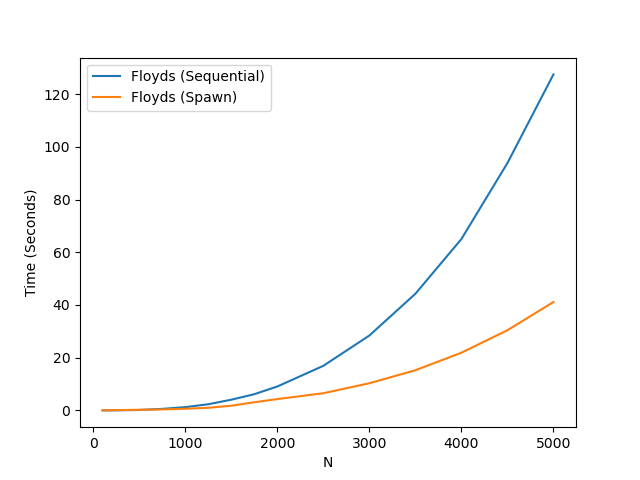
\includegraphics[width=9cm]{images/benchspawn2.png}
    \caption{Parallel Floyd's-Spawn with 20 threads versus sequential Floyd's}
    \label{fig:floyds_spawn}
\end{figure}

We can observe in figure \ref{fig:floyds_spawn} a roughly 3x speedup with 20 threads with this method. We will go in greater detail with the effects of thread count on running time later. 

The main potential problem with this solution is the overhead of repeatedly creating and destroying threads for every iteration of the "K loop". We can fix this problem by creating the worker threads once and re-using them, but we will have to make sure that one worker thread does not move ahead to the next value of k before every other thread has finished with the same thread. We can accomplish this by having each thread increment a counter when it finishes for some k, and then wait (by locking a mutex). Then, when this counter reaches the number of threads, every thread can be unlocked and continue on to the next value of k. This process will repeat for $n$ iterations. We will call this approach "Floyd's-Sync", since all the threads are "syncing" before moving on together to the next value of k (after which they might fall out of sync until finishing). The c++ implementation for this approach is shown in listing \ref{lst:syncfloyds}.

\begin{figure}[t]
    \lstinputlisting[
        language=C++,
        caption=Floyd's-Sync implementation,
        label=lst:syncfloyds
    ]{./src/APSP/floyds_sync.cpp}
\end{figure}

\begin{figure}[t]
    \centering
    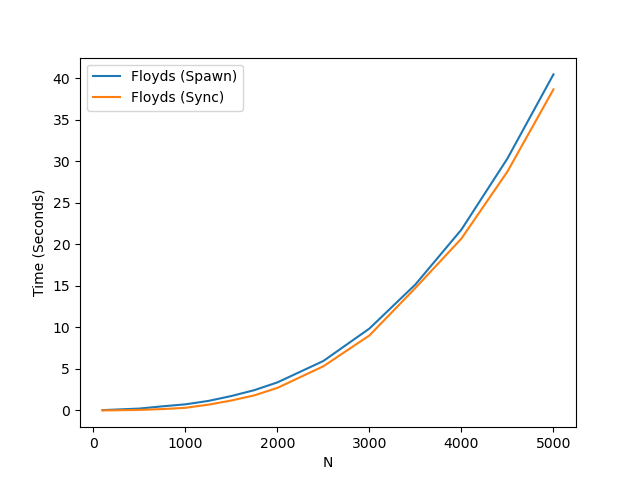
\includegraphics[width=9cm]{images/benchsync.png}
    \caption{Floyd's-Sync versus Floyd's-Spawn, both with 20 threads}
    \label{fig:floyds_both}
\end{figure}


Again, running this implementation against the others which are working as intended, this implementation also produces correct output. Figure \ref{fig:floyds_both} shows Floyd's-Sync and Floyd's-Spawn run on the same inputs, and while the improvement is only marginal, Floyd's-Sync is consistently slightly faster than Floyd's-Spawn.

\subsection{Dijkstra's Algorithm in Parallel}\label{AA}
In the previous section, we analyzed different practices for computing the All-Pairs-Shortest-Path matrix in parallel using Floyd-Warshall's algorithm. The other algorithm we will be considering for computing this matrix will be All-Sources Dijkstra's algorithm; that is, we will run Dijkstra's from every node as a source. If we observe the implementation shown in listing \ref{lst:seqdijkstra}, we will notice that, for any function call of $dijkstra$ on an arbitrary starting point $s$, the only changes that can be seen from outside the method are in the row $res[s]$. This suggests an implementation of All-Sources Dijkstra's in parallel: Call $dijkstra(i)$ on every node. As observed previously, we won't have any issues like we had in the previous section with Floyd's, as any updates are constrained to a single row in the result matrix, and function calls to $dijkstra$ are ambivalent to any changes made in any row except for the row of the starting node. Thus, we do not expect any issues, and can code a relatively straightforward parallelization shown in listing \ref{lst:pqdijkstras}.

\begin{figure}[t]
    \lstinputlisting[
        language=C++,
        caption=Trivial Dijkstra's parallelization,
        label=lst:pqdijkstras
    ]{./src/APSP/dijkstra_pq.cpp}
\end{figure}

\begin{figure}[t]
    \centering
    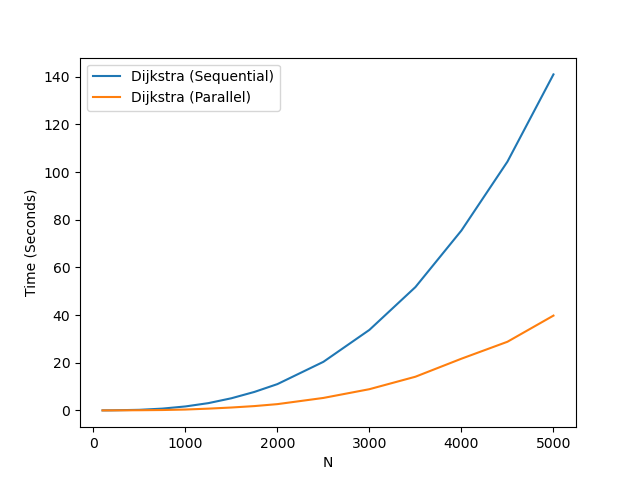
\includegraphics[width=9cm]{images/benchpq.png}
    \caption{Sequential vs Parallel Dijkstra's APSP with 20 threads}
    \label{fig:dijkstra_pq}
\end{figure}

\begin{figure}[t]
    \lstinputlisting[
        language=C++,
        caption=Dijkstra's with Linear Search instead of Priority Queue
        label=lst:lineardijkstras
    ]{./src/APSP/dijkstra_linear.cpp}
\end{figure}



\begin{figure}[t]
    \centering
    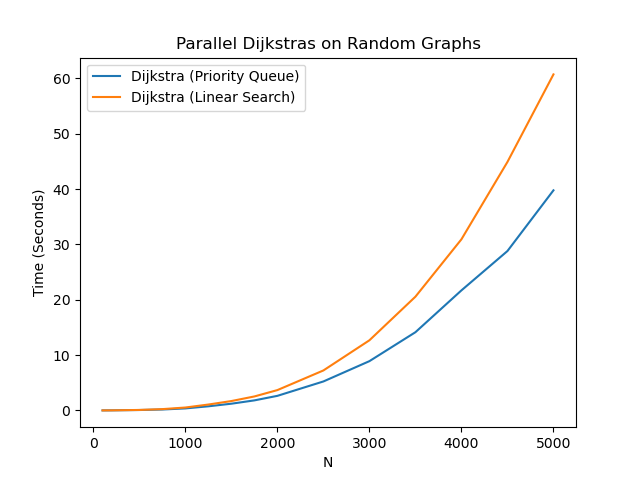
\includegraphics[width=9cm]{images/benchdijkstra.png}
    \caption{Dijkstra's with Priority Queue vs Dijkstra's with Linear Search on randomly-generated graphs, both with 20 threads}
    \label{fig:dijkstra_both}
\end{figure}

\break
\newpage

\section{Minimum Spanning Tree}
The Minimum Spanning Tree (MST) problem is a common architecture building problem that finds the minimum-weighted connected graph of a certain set of connected vertices. The graph will contain V-1 edges where V is the total number of vertices in the graph. This problem can be found in many real life problems such as road construction, circuit design & development, and phone line planning. In the realm of computer science research the MST problem can also be used to approximate NP-Hard problems such as the traveling salesperson. We will be looking at how to properly implement a solution concurrently and compare the runtimes to the sequential implementation.

\subsection{Prim's MST}
Prim's MST is a greedy approach to the MST problem where the concept is to maintain two sets of vertices: the set of vertices included in the tree, and the vertices yet to be added. As the tree is built, each edge between the two sets are considered and the smallest weighted edge is chosen to be a part of the tree. The minKey function takes in the two sets and returns the index of the minimum weighted edge that connects the two. The sequential implementation can be seen below:

\lstinputlisting[
    language=C++,
    caption=,
    label=,
]{./src/MST/prims_seq.cpp}

\section{Single-Source Shortest Path with Negative Edge Weights}
What this research hopes to address is the problem of finding shortest path distances in a directed weighted graph from a single source with the additional complication of allowing negative edge weights. We will also address the problem of finding negative sum cycles in such graphs. The two most known algorithms that are applicable to this problem are the Bellman-Ford algorithm and the Floyd-Warshall algorithm. We will explore the parallelization of these algorithms in relation to this problem and their performance.

\subsection{The Bellman-Ford Algorithm}\label{AA}
WIP

\lstinputlisting[
    language=C++,
    caption=,
    label=
]{./src/bellman_ford.cpp}

\section{The Disjoint Set Union Problem}

\subsection{Problem Definition}
The Disjoint Set Union, alternatively called the Union Find Problem, is to maintain several disjoint sets with the ability to merge these disjoint sets together and determine if different items are in the same set. This can be achieved by maintaining a unique representative for each disjoint set. When we union two sets, we make the representative of one set the representative of the other set, thus uniting the sets into one.

Such a data structure that can do this should support the following operations: \\ \\
$find(x)$: Find and return the representative of the set that contains $x$. \\ \\
$unite(x, y)$: Get the representative of the set containing $x$ and the representative of the set containing $y$. If the representatives are the same, they are in the same set, otherwise, combine the sets by setting the representative of one of the two representatives to the other. \\ \\
All sets begin only containing it's index, with it's representative being the index. We will also include the following operations: \\ \\
$sameSet(x, y)$: Determine if $x$ and $y$ are in the same set by getting their respective representatives and comparing if they are the same or not.

\subsection{Sequential Implementations}

We will examine naïve implementations of $find(x)$ and $unite(x, y)$, and go over the different optimizations that can be applied to them to improve overall time complexity. As we go along the path of representatives, we will call the next representative the parent, and the representative of the set the root.

\lstinputlisting[
    language=C++,
    caption={Naïve implementation of $find(x)$.},
    label=lst:naivefind
]{./src/DisjointSetUnion/dsu_find.cpp}

\lstinputlisting[
    language=C++,
    caption={Naïve implementation of $unite(x, y)$.},
    label=lst:naiveunite
]{./src/DisjointSetUnion/dsu_unite.cpp}

These implementations have problems because we have no rules on how we designate who becomes the root of who. We can see here that in the worst case, we can create a long chain of parents, which would make the worst case of $find(x)$ be $O(n)$, with no improvements to happen over time. There are several optimizations that we can do to improve the time complexity. We will first look at linking by size, linking by rank, and linking by random index.

When we link by size, the idea is to maintain the size of each disjoint set, and use the sizes to determine what the new root will be in $unite(x, y)$. When we go to try and unite the two sets, we will make the root of the set that has a larger size be the root of the new combined set. Ties are broken arbitrarily.

\lstinputlisting[
    language=C++,
    caption={Implementation of $unite(x, y)$ with linking by size.},
    label=lst:unitelinkbysize
]{./src/DisjointSetUnion/dsu_unite_link_by_size.cpp}

When we link by rank, the idea is to maintain the length of the longest path from the root to any other value in the set. When we $unite(x, y)$, we make the root with the higher rank the root of the new combined set. If there is a tie, we arbitrarily choose the root of the new set, and increase the rank by 1.

\lstinputlisting[
    language=C++,
    caption={Implementation of $unite(x, y)$ with linking by rank.},
    label=lst:unitelinkbyrank
]{./src/DisjointSetUnion/dsu_unite_link_by_rank.cpp}

When we link by random index, the idea is to create a random ordering of the values, and use the position in the ordering to determine who becomes the root. The root with the later position in the ordering becomes the root of the combined set. Since each position is unique, there will never be ties.

\lstinputlisting[
    language=C++,
    caption={Implementation of $unite(x, y)$ with linking by random index.},
    label=lst:unitelinkbyrandomindex
]{./src/DisjointSetUnion/dsu_unite_link_by_random_index.cpp}

Another point of improvement that can be made is that if the parent of $x$ is $y$ and the parent of $y$ is $z$, since we only care about the root of the whole set, we can get rid of this chain by simply making it so that parent of $x$ is $z$. There are several optimizations for achieving this, being compression, halving, and splitting.

When we do compression, we simply make all the parents on the path are set to the root.

\lstinputlisting[
    language=C++,
    caption={Implementation of $find(x, y)$ with compression.},
    label=lst:findcompression
]{./src/DisjointSetUnion/dsu_find_compression.cpp}

When we do halving, we replace the parent of every node on the path with it's grandparent.

\lstinputlisting[
    language=C++,
    caption={Implementation of $find(x, y)$ with halving.},
    label=lst:findhalving
]{./src/DisjointSetUnion/dsu_find_halving.cpp}

When we do splitting, we replace the parent of every other node on the path with it's grandparent.

\lstinputlisting[
    language=C++,
    caption={Implementation of $find(x, y)$ with splitting.},
    label=lst:findsplitting
]{./src/DisjointSetUnion/dsu_find_splitting.cpp}

\begin{thebibliography}{00}
\bibitem{b1} G. Eason, B. Noble, and I. N. Sneddon, ``On certain integrals of Lipschitz-Hankel type involving products of Bessel functions,'' Phil. Trans. Roy. Soc. London, vol. A247, pp. 529--551, April 1955.
\bibitem{b2} J. Clerk Maxwell, A Treatise on Electricity and Magnetism, 3rd ed., vol. 2. Oxford: Clarendon, 1892, pp.68--73.
\bibitem{b3} I. S. Jacobs and C. P. Bean, ``Fine particles, thin films and exchange anisotropy,'' in Magnetism, vol. III, G. T. Rado and H. Suhl, Eds. New York: Academic, 1963, pp. 271--350.
\bibitem{b4} K. Elissa, ``Title of paper if known,'' unpublished.
\bibitem{b5} R. Nicole, ``Title of paper with only first word capitalized,'' J. Name Stand. Abbrev., in press.
\bibitem{b6} Y. Yorozu, M. Hirano, K. Oka, and Y. Tagawa, ``Electron spectroscopy studies on magneto-optical media and plastic substrate interface,'' IEEE Transl. J. Magn. Japan, vol. 2, pp. 740--741, August 1987 [Digests 9th Annual Conf. Magnetics Japan, p. 301, 1982].
\bibitem{b7} M. Young, The Technical Writer's Handbook. Mill Valley, CA: University Science, 1989.
\bibitem{b8} S. V. Jayanti and R. E. Tarjan, ``Concurrent Disjoint Set Union,'' Distributed Computing, vol. 34, pp 413-436, Dec 2021.
\end{thebibliography}
\vspace{12pt}
\color{red}
IEEE conference templates contain guidance text for composing and formatting conference papers. Please ensure that all template text is removed from your conference paper prior to submission to the conference. Failure to remove the template text from your paper may result in your paper not being published.

\end{document}